\section{Adopted solutions}

\subsection*{Part A: Clustering}
This part is conducted in an unsupervised approach, with the idea of grouping
sentences with clustering algorithms. In particular, we used the
\textbf{sklearn} library, with the AgglomerativeClustering class as
suggested.\\ The main paths to explore in this part are:
\begin{itemize}
    \item \textbf{Number of clusters and used metrics: }  the main challenge here was the correct choice of the \textbf{number of clusters}, because it's a parameter than could have a big impact on the results. Using \textbf{silhouette score } we have solved this problem in a iterative way.
    \item \textbf{Sentences selection: } the second challenge was to select the sentences that would be used to build the summary. Using \textbf{centroids} of each clusters, we were able to build summaries that had more topics and were more representative of the original text.
\end{itemize}

\subsubsection*{Number of clusters and used metrics} 
A problem related to part A is to define a good number of clusters to represent the feature space of the document.\\
In this part, we tried to construct a custom metric taking into account Silhouette score, Calinski-Harabasz score and a function of the number of clusters. The idea was to consider the number of clusters, that can vary in the range $[2,numberOfSentences]$, to avoid high sparse clusters representation with single-sentence clusters, but in the end we noticed that the silhouette score by itself was performing overall better.\\We are leaving the code for the custom metric in the notebook, but it is commented since it was not used in the final version of the code.\\

\subsubsection*{Sentences selection}
Another relevant problem, once completed the clustering part of the project, was to decide the criteria to pick the sentences to use in the summarization. We decided to use the \textbf{centroid} of each cluster and, based on the distance from it, we pick the required number of sentences. We have done some tests on different criteria, but others ideas that we had were not really convincing on summaries, so we kept the centroid distance as metric.\\ It is important to note that this strategy has a limitation, since with high numbers of sentences picked from each cluster there might be some redundancy in summaries. Nevertheless, with a low number of picked sentences it is leading to convincing results, taking into the summary relevant sentences.
\subsection*{Part B: Classification}
In this section the task is to create a binary classifier that has as goal to discern if a sentence should belong to the summary or not. We used models from the \textbf{scikit-learn} library, and in particular the machine learning techniques that we exploded are Random Forest, Gradient Boosting, Gaussian Naive Bayes, K-Neighbors and Multi-layer Perceptron. \\
Before the training phase, the challenge was to find the best features and the correct shape to represent data and build the models. Since the classifier should classify sentences, each row of our dataset represents one sentence in the original library. We ended up with the following structure.\\ 
\begin{table}[H]
    \resizebox{\textwidth}{!}{%
    \begin{tabular}{|c|c|c|c|c|c|c|c|c|}
        \hline
        similarity & n\_sentence & n\_words & n\_stopwords & n\_keywords & length\_of\_sentence & tfidf\_score  \\ \hline
        position\_in\_doc & category & n\_nouns & n\_verbs & n\_adjectives & n\_adverbs & id \\ \hline
        summary(target) &  &  &  &  &  &  \\ \hline
    \end{tabular}%
    }
    \end{table}
We then analyzed the features with a correlation matrix, the Shapley value of each features via the \textbf{SHAP} library and the Scikit-learn built-in feature importance. This process lead us to drop some features, with the following schema being the one used to train our models. 
    
\begin{table}[H]
    \resizebox{\textwidth}{!}{%
    \begin{tabular}{|c|c|c|c|c|c|}
    \hline
    similarity & n\_sentence & n\_words & n\_stopwords & n\_keywords & length\_of\_sentence \\
    \hline
    tfidf\_score & position\_in\_doc & n\_nouns & n\_verbs & n\_adjectives & n\_adverbs \\
    \hline
    category\_business & category\_entertainment & category\_politics & category\_sport & category\_tech & Summary(target) \\
    \hline
    \end{tabular}%
    }
    \end{table}
At this point, we could train our models and evaluate them with the common machine learning evaluation metrics. The one performing better is, in our case, RandomForest.\\More on this can be found in the notebook, as well as in the following chapter.

\begin{figure}[H]
    \centering
    \begin{subfigure}{0.45\textwidth}
      \centering
      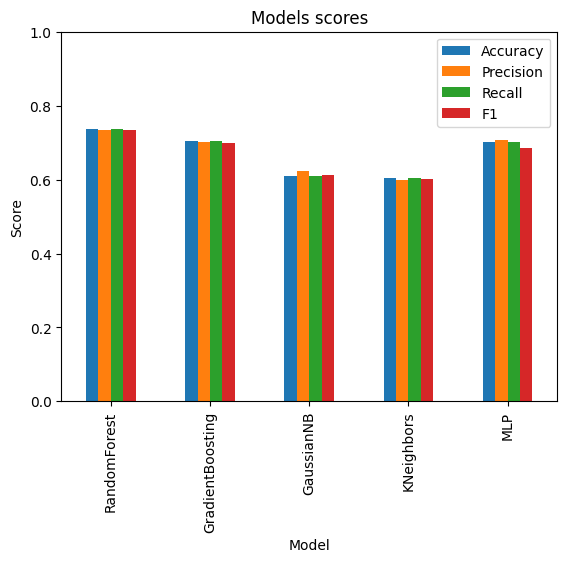
\includegraphics[width=\textwidth]{images/models_scores.png}
      \caption{Models scores comparison}
      \label{fig:immagine1}
    \end{subfigure}
    \hfill
    \begin{subfigure}{0.45\textwidth}
      \centering
      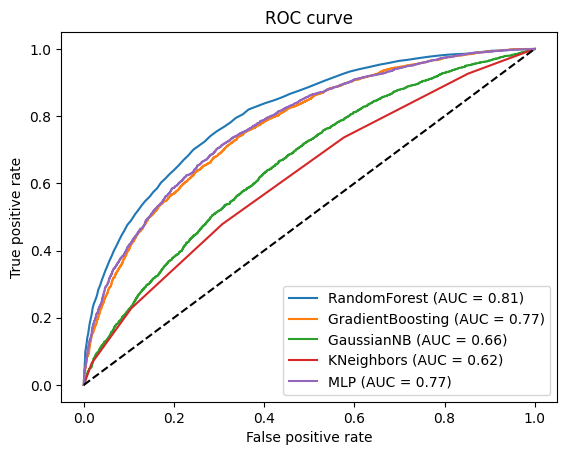
\includegraphics[width=\textwidth]{images/roc_curves.png}
      \caption{Models ROC curves comparison}
      \label{fig:immagine2}
    \end{subfigure}
    \caption{Descrizione generale delle immagini}
    \label{fig:immagini}
  \end{figure}